\section{Procesja do Bożego Grobu}

\begin{itemize}
	\item ministranci rozdzielają świece i zapalają je
	\item \tt1 i \tt2 wychodzą z kadzielnicami, \oo~ bierze ombrelino, \ding{63}
	      bierze krzyż i staje u wejścia do prezbiterium
	\item \aa2 przynosi na ołtarz monstrancję i przejrzysty welon do niej,
	      podczas gdy \cc3 zabiera mszał wraz ze stojakiem.
	\item \ii~ wraz z \cc1 i \cc2 podchodzi do stopni ołtarza, przyklęka i sam
	      wchodzi na górę
	\item po wystawieniu NS \ii~ schodzi przed stopnie, zasypuje kadzidło
	      i okadza NS
	\item po okadzeniu \aa2 nakłada \ii~ welon naramienny i razem z \aa1
	      zabierają akolitki z kredencji, z którymi ustawiają się obok \ding{63}
	\item \kolatki1 i \kolatki2 biorą kołatki
	\item duchowieństwo wkłada {\color{violet} fioletowe} stuły
	\item gdy \ii~ bierze monstrancję, \cc3 formuje procesję w kolejności:

	      \begin{center}
		      (stopnie ołtarza) \smallskip\\
		      \oo \smallskip\\
		      pochodnie~~\cc1~~\ii~~\cc2~~pochodnie \smallskip\\
		      \tt1~~\tt2 \smallskip\\
		      \kolatki1~~\kolatki2 \smallskip\\
		      duchowieństwo \smallskip\\
		      ministranci ze świeczkami (w parach) \smallskip\\
		      \aa1~~\ding{63}~~\aa2 \smallskip\\
		      \downarrow
	      \end{center}

	\item procesja idzie następującą drogą (patrz Rys. \ref{fig:procesja1_pt}):

	      \begin{figure}[h]
		      \centering
		      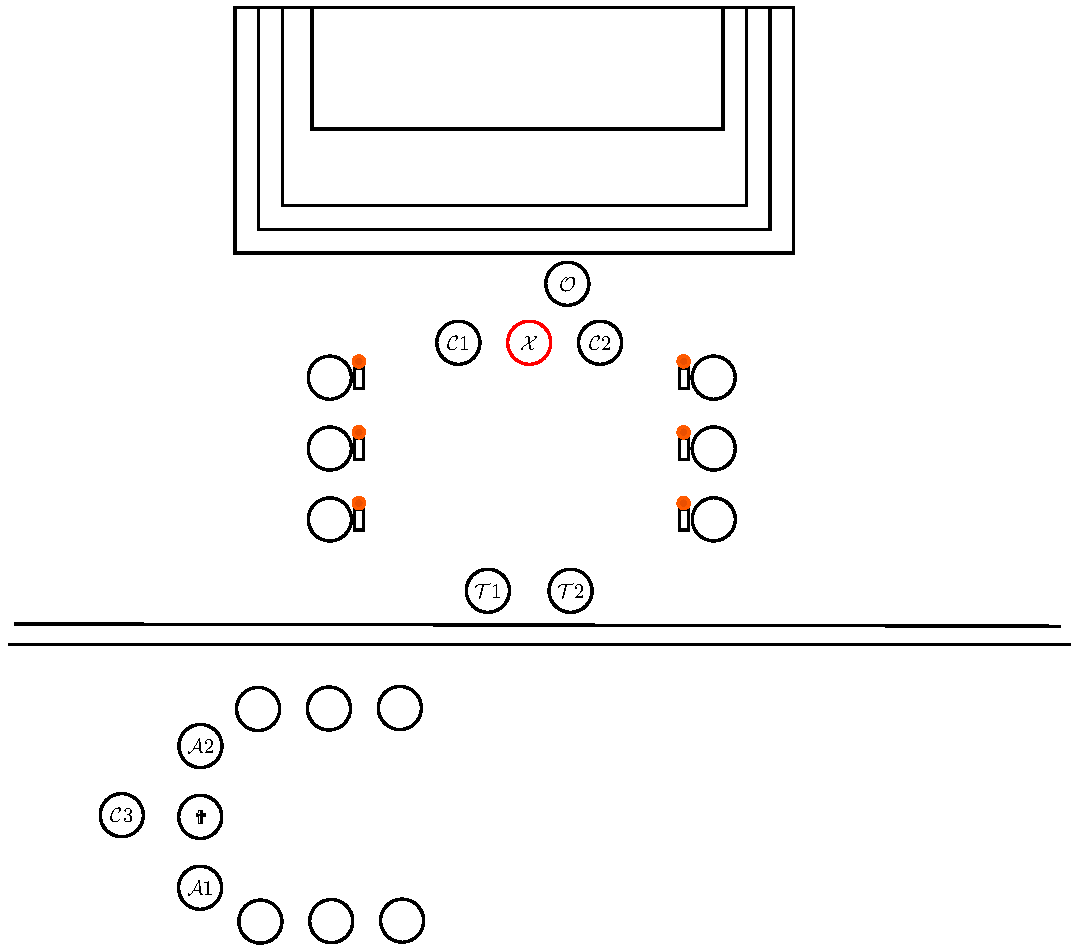
\includegraphics[scale=0.6]{Piatek/Procesja1.pdf}
		      \caption{Droga procesji}
		      \label{fig:procesja1_pt}
	      \end{figure}

	\item po dokonaniu wystawienia w Bożym Grobie następuje zasypanie i
	      okadzenie, a następnie krótka adoracja w ciszy
	\item asysta wychodzi procesjonalnie do zakrystii (patrz Rys. \ref{fig:procesja2_pt})

	      \begin{figure}[t!]
		      \centering
		      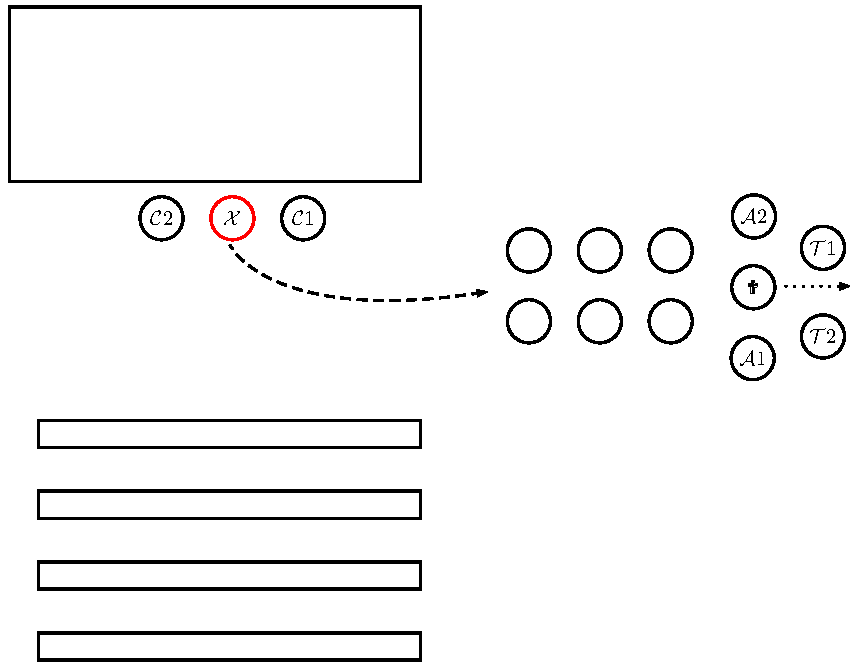
\includegraphics[scale=0.7]{Piatek/Procesja2.pdf}
		      \caption{Procesja do zakrystii}
		      \label{fig:procesja2_pt}
	      \end{figure}

	\item \ii~ lub członek duchowieństwa w asyście dwóch pochodni i \oo~, z welonem
	      na ramionach przenosi puszkę z tabernakulum do Bożego Grobu
	\item po liturgii na ołtarzu zostają tylko 4 świeczniki i krzyż
\end{itemize}

